\documentclass{article}

\usepackage{microtype}
\usepackage{graphicx}
\usepackage{subfigure}
\usepackage{booktabs}
\usepackage{hyperref}
\usepackage{svg}

% If your build breaks (sometimes temporarily if a hyperlink spans a page)
% please comment out the following usepackage line and replace
% \usepackage{icml2018} with \usepackage[nohyperref]{icml2018} above.

\usepackage{icml2018}

\author{
  Duggan, WIll\\
  \texttt{dwduggan@mail.sc.edu}
  \and
  Lewis, Cole\\
  \texttt{lewiscg@mail.sc.edu}
  \and
  Mallari, Daniella\\
  \texttt{dmallari@mail.sc.edu}
}
\title{}

\begin{document}
\twocolumn[
\icmltitle{Audio-Visual Fusion Assisted Disaster Rescue}           
\maketitle

\vskip 0.3in
]

% abstract
\begin{abstract}
As the Earth’s climate changes, our species is experiencing a rapid increase of volatile and dangerous weather events that often tragically conclude in disaster where a great loss or injury of life and property is experienced. This is happening more frequently in more areas now than ever before. We are attempting to solve the problem of how best to effectively navigate disaster-stricken environments safely, effectively, and quickly to determine where rescue resources should be allocated most efficiently towards locating and saving victims. To meet this challenge, we developed a system that implements fusion of both a visual, human-detection model and an audial, human-generated sound-detection model to determine potential victims within the immediate surroundings. The results at this stage of development proved to be a foundation upon which future work can be done, however, are underwhelming given available hardware, time constraints, and naive method of sound source localization.

\end{abstract}

% use sections to delineate paper
\section{Introduction}
The problem at hand that we are attempting to solve is how to safely, efficiently, and quickly locate disaster victims within volatile and dynamic environments after a disaster has occurred. Conditions such as building or infrastructure collapse, immobilization or injury, as well as other obstacles that may impede camera input such as smoke or dust all contribute towards the need for a holistic, “multi-sensory” approach that requires multiple forms of input in the search for victims. We set out to accomplish this in our project by fostering within our system a dependence upon both audio and visual inputs from a microphone and camera respectively in order to make positional inferences. This is done through having our human-generated sound-detection model check detection results from our computer-vision, human-detection model to better make inferences as to where a potential disaster rescue victim may be located relative to the microphone and camera apparatus. Directional inference is then performed if our sound detection model determines that it detected somebody. The loudest average input channel is then found and mapped to a cardinal direction before being written to standard output. 

\section{Contextual Work}
As inspiration for our project, and to support our idea of implementing different stimuli for the robot, we used the following existing projects. The PERCEPTION team at INRIA Grenoble Rhône-Alpes published their studies on Audio-Visual Fusion for Human-Robot Interaction for their companion robot NAO, showcasing their experience with visual, audio, and visual-audio processing in order to have the robot be able to analyze a scene using omnidirectional microphones and high definition cameras. Similar to our project, the idea of fusing two different data inputs in order to achieve a higher level of interpretation was the focus of the PERCEPTION team’s study. Since their application was for a companion robot, their models were being trained on human activity, specifically person detection, pose, and gaze of the subject or subjects being observed in order for their robot to respond accordingly. While our application is for disaster rescue, our models are also concentrated on humans, for instance our visual model would be trained on various human body parts in the case of an obscured victim behind debris and our audio model would be trained for human sounds such as shouts and yells. Compared to the PERCEPTION team’s project, ours would use the same data inputs and fusion of visual and audio data, but would be more focused on finding humans than trying to figure human activity and intent.The SoundSpaces Platform is a project focused on building and implementing embodied agents in artificial intelligence to use audio and visual data to navigate 3D environments. The project offers datasets of audio renderings from visually and acoustically realistic simulations using sets of 3D environments. This initially provided inspiration to our team about pursuing acoustic beamforming alongside a dedicated neural network as a means of sound source localization, however, given the time, knowledge, and hardware constraints as well as a lack of standard environment with which to initialize our model for beamforming, we adopted alternative measures.


\section{Data}
Given that there are two different models, two different sets of data are used. The visual model is pre-trained on an object-detection dataset with labeled people. The data in this dataset are labeled images. The labels included the class of the object as well as bounding-box labels for where the person is in the frame. Before being passed to the model, the pixel values of each frame are standardized to a scale between 0 to 1. A standardized scale during training of the model allows the model to converge faster.
The sound classification task used a combination of two different datasets, the ESC-50 [CITATION FOR DATASET] environmental sound classification dataset and some samples from the 8k Flickr audio corpus [CITATION FOR DATASET]. The ESC-50 dataset consisted of samples of 50 different semantic classes ranging from cow, to mouse clicking, to helicopter. 10 of these classes were considered “human, non-speech sounds” {ESC-50}. Each class contained 40 recordings, 5 seconds in length and sampled at 16kHz. Using these samples meant that there were 400 examples of non-speech human sounds and 1600 samples of non-human environment sounds. To create a dataset with two equally weighted classes, examples from the 8k Flickr audio corpus were added to the human sounds class so that both classes had 1600 samples. The 8k Flickr audio consists of recordings of speakers captioning multiple images verbally with no particular length, sampled at 16kHz. The data for the sound classification model was preprocessed before training. To ensure that there was no error in the lengths of the recordings, Librosa was used to load and resample the audio clips to a consistent 16kHz. The average length of the recordings was found to be ~54000 samples. Librosa was again used to cut each recording to a consistent length of 64000 samples based on the average found. The samples were then converted to spectrograms to be used for classification in the sound classification model. The spectrograms were then converted to grayscale and resized to a height and width of 128 pixels. The purpose of this was to decrease the amount of information that would need to be processed by the network and to have consistent input sizes.

\section{Methodology}
Our project consists of two models which interact via a shared buffer of timestamps to determine if somebody was detected by the camera and our sound model simultaneously. In Figure 3 below, we outline and detail how each component works together before explaining how each component works individually.

\begin{figure}[ht]
\begin{center}
\centerline{\includegraphics[width=\columnwidth]{full_diagram}}
\caption{High level overview of our entire system and how each model is integrated with each other.}
\end{center}
\end{figure}

\subsection{Visual Recognition Model}
Originally, we had sought to develop an object-detection model using YOLOv3 and TensorFlow that would be trained to recognize various human body parts, to ensure that human detection would not only be limited to instances in which a full body shot can be taken. We chose to use the YOLOv3 algorithm because it is well implemented and well documented. As time went on and we experimented with training runs of the model, we realized that training that model would be a challenge. One reason for this was because our group had to use an existing implementation of the model. YOLOv3 is built off of a Darknet backbone, which is implemented in C++. This made re-implementing the model a challenge for our group, so we chose to use an existing implementation. This came with its own set of challenges though, as if we wanted to retrain the model, we would have to change our data to fit with the implementation. YOLOv3 implementations are also a couple of years old, meaning that there were also many bugs that needed to be fixed from libraries that had changed over time. After fixing the bugs and getting the training to run, we had issues finding hardware that could train the model within a reasonable time. Training on a laptop took approximately 12 hours for 50 epochs, which was far slower than needed. Additionally, many training runs would need to be performed with different hyperparameters to find an optimal model. When moving to a cloud GPU environment, Chameleon, to continue training with faster hardware, the size of the dataset and millions of parameters contained within the model proved yet again far too slow to train, taking approximately 15 hours to train each iteration with the provided GPU. After having trained the model a few times on Chameleon, we realized that the time spent struggling was not worth the possibility of a completely non-functional visual detection model.
Our team found a pre-trained human detection YOLOv4-tiny model in our research [model link] that proved capable of consistently detecting people at a high enough speed that we felt confident it could stand up to the task. Having already been quantized and in TFLite format as well as able to detect people even when only viewing an arm or leg, this model accomplished what we had set out to do as well as assuage any fears of being limited by people being completely. This model has clear advantages over the model we were developing in that it is faster, able to make inferences at approximately 16-17 frames per second when using the PlayStation Eye and a laptop with a Radeon Pro 560X graphics processing unit, rather than the approximately 11-12 frames per second previously. This performance gain is likely to prove even greater when deployed on hardware dedicated to running machine learning models.

\subsection{Human-generated Sound Detection Model}
The purpose of the human-generated sound detection model is to classify whether sounds recorded by the microphone are created by a human or not. Classifying the sound of sounds helps the sound-source localization of our system because it makes the system tolerant to irrelevant background noises and other noises that do not aid the search for human victims. As mentioned in the Data section above, the model was trained on a mix of human, non-speech speech sounds and human speech recordings. This gave the model a mix of different human-based sounds to classify as being of human-origin.
The model used for the sound classification was a simple Convolutional Neural Network (CNN). We chose to utilize a CNN and spectrograms instead of a sequence-based model such as a Recurrent Neural Network (RNN) based on its simplicity and demonstrated success [paperspace][towardsData]. The architecture of the model is shown in Figure 2 below.

\begin{figure}[ht]
\begin{center}
\centerline{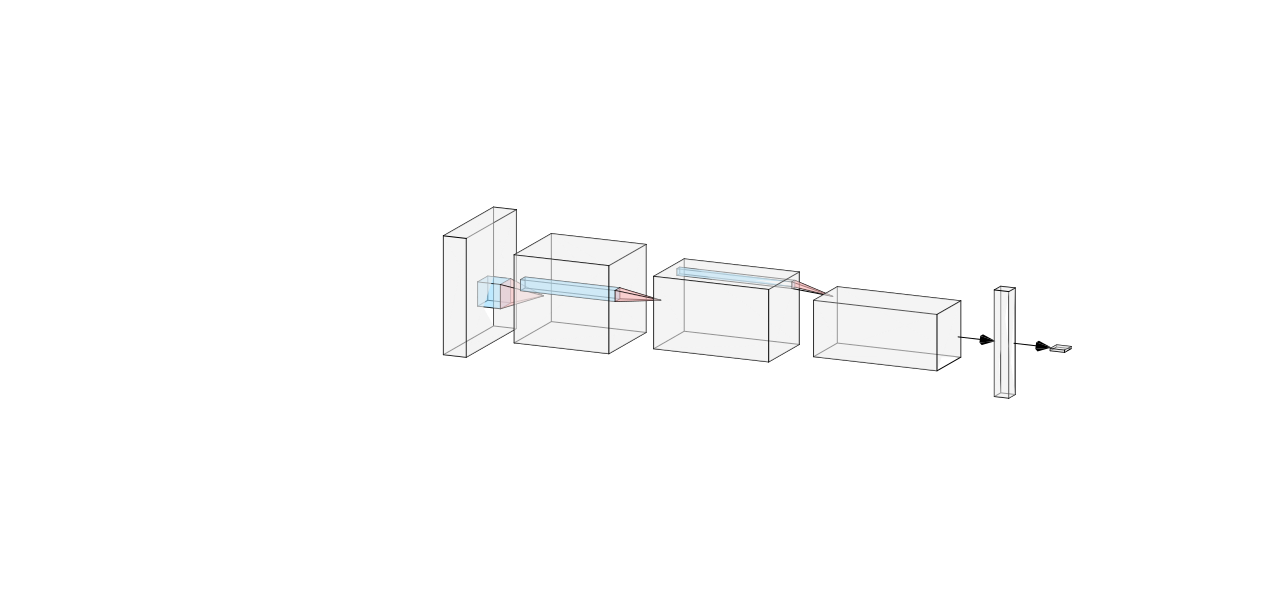
\includegraphics[width=\columnwidth]{nn_diagram}}
\caption{Diagram of the convolutional neural network for the human-generated sound detection model. In order is the convolutional layer, a pooling layer, a secondary convolutional layer, another pooling layer, a fully connected layer, then finally an output layer.}
\end{center}
\end{figure}
The human-generated sound detection model consists of two convolutional layers and two pooling layers with kernel sizes and filters listed above. These blocks extract features from the input spectrogram and only keep the most relevant features. The filters are learned through the training of the network, and reflect features of human-generated speech spectrograms. After the convolution and pooling, the input is flattened and passed through a fully-connected layer and finally, to the output neuron. ReLU [CITATION] activations are used in between each of the layers except in-between the fully-connected and the output, which uses a sigmoid activation [CITATION FOR SIGMOID]. A sigmoid activation was used to force the output to be a probability that the input sample was a human-generated sound. Batch normalization [CITATION] was also used after each pooling layer. An output of 1 means that the model is completely confident that the sound was a human-generated sound, and an output of 0 means the model is completely confident that the sound was not of human-origin.

\subsection{Model Integration and Fusion}
Both models are integrated by way of a buffer of timestamps that contains 110 entries. The visual detection model writes a Unix timestamp to the buffer on each frame that a person is detected. Once the buffer is full, the oldest entries become overwritten by new timestamps, ensuring that we only capture the prior 6-7 seconds depending on the frame rate that our model is performing at. The buffer size will need to be adjusted when deploying our system on more capable hardware to provide at least 7 seconds of buffer time. 7 seconds of buffer time easily allows for the 5 seconds of sound recording done by the human-generated sound detection model, an approximate 0.2 seconds for our sound model to make an inference, and an additional 1.8 seconds to account for any anomalous slowdowns that may occur due to model caching, system load, or other such conditions. Below is an equation to determine an appropriate buffer size B, in entries, dependent on the frame rate at which the visual detection model performs, denoted by F.

\begin{math}
B = F / 7
\end{math}

If our human-generated sound detection model detects a person, it will then compare a Unix timestamp dating to the sound recording file’s creation time to the contents of the buffer to determine if it is present. If present, the system assumes that the person was in view of the camera and detected by the sound model, allowing a prediction to be made that a person is in front of the PlayStation Eye. Otherwise, if a person was detected audibly, but not visually, we then use our means of sound source localization, taking the channel whose amplitude was highest on average over the recording duration, to predict the position of the person relative to the microphone array already knowing they were not in front of the apparatus. A predicted position, relative to the PlayStation Eye, and its associated confidence level are then printed to a terminal’s standard output before another 5 second recording is made, and the process continues indefinitely. 

\section{Experiments}
We subjected our system to a test consisting of 20 trials set in a near-silent environment in which a test subject spoke at a consistent distance of approximately one meter at varying cardinal directions to gauge both the accuracy of the sound-recognition model and our means of sound source localization. We ran the test for 20 trials using two distinct methods of sound source localization: inferring which direction the sound originated from by selecting the channel whose amplitude was the highest at any given point in the five-second interval, and selecting the channel who at any given point in the recording detected the highest amplitude. The results of this test are shown in Figure 3, displaying the accuracy of the entire system as a whole throughout the test on both sound source localization methods. Results were further broken down by the accuracy of our sound model alone, determined by whether or not it could correctly classify the test subject’s voice as human-generated or not, and are shown in Figure 4.
\begin{figure}
\begin{center}
\centerline{\includegraphics[width=\columnwidth]{localization_test}}
\caption{Sound source localization experiment. On the y-axis is the number of trials in which the system successfully detected which our test subject stood and spoke from, and on the x-axis is labeled which method was used.}
\end{center}
\end{figure} 
\begin{figure}
\begin{center}
\centerline{\includegraphics[width=\columnwidth]{sound_model_accuracy_chart}}
\caption{Sound source localization experiment. On the y-axis is the number of trials in which the system successfully detected which our test subject stood and spoke from, and on the x-axis is labeled which method was used.}
\end{center}
\end{figure}


A further experiment was conducted to find the average time it takes for our human-generated sound detection model to make inferences. After determining that making inferences takes an equal amount of time regardless of the result, we had the model make inferences over a 5 second recording of our test subject tapping the microphone array 1000 times. The results were an average inference time of 0.1989 seconds with a standard deviation of only 0.02 seconds.
Unfortunately the sound model and means of sound source localization both performed poorly. However, there are many factors at play which we believe contributed to the overall performance of our system, further evidenced by a 74\% accuracy rate of the sound model when making inferences over its test set. The greatest consideration is that of the hardware upon which our system was implemented. The PlayStation Eye was designed in 2007 as an accessory to the PlayStation 3. Alongside a camera, the PlayStation Eye contains a 4-microphone, omnidirectional, linear array with a maximum sample rate of 16 kHz, far lower than the industry standard of even a CD, which stands at 44.1 kHz. Acoustic hardware is very nuanced and liable to be influenced by minute factors that require identical conditions to replicate; the training set for our sound model was carefully curated to provide an accurate benchmark for human and non-human sounds alike, likely with much better recording hardware and in more advantageous conditions. The size of the microphone array, only 76 mm in width, only gives each microphone approximately 19 mm of distance apart from each other when accounting for the size of the casing. The PlayStation Eye’s limited size and relatively simple audio controller provides the ideal environment for each microphone to lose independence as sound input becomes muddled as to which microphone is uniquely detecting a specific sound.The performance of the system as a whole depends on the performance of each component, as directional inference fails without the accurate function of both the visual and audial model. The failure of a single model or detection cascades across the entire system and renders it ineffective.


\section{Conclusion}
\subsection{What Was Learned}
Over the course of this project, our team primarily gained a thorough understanding of adapting existing machine learning models, and developing our own. Our team opted to design and use TensorFlow at each step due to the large body of documentation present and ease of use when first learning how to implement, train, manipulate, and generate inferences from machine learning models. More fundamentally, our team learned core fundamentals pertaining to neural networks and the process of their construction and use, aided by in-class lectures and supplementary assignments. This extends to learning done for Keras, a high-level neural network library, which runs on top of TensorFlow.
Obtaining a grasp of assembling and preprocessing data sets, the Python implementation of OpenCV, and interfacing with microphones were necessary to complete the project. We are confident that the knowledge we developed will persist and continue to be useful with future machine learning projects.
\subsection{Future Improvements}
First and foremost, we believe that the best future improvements to our project come in the form of better hardware, especially for the microphone. This would address many of the difficulties we describe in the Results section. Furthermore, with time comes a deeper and more thorough knowledge of how better to optimize both the models and their implementations. What comes to mind immediately would be quantizing and pruning our human-generated sound detection model to reduce inference time and disk space utilized by the model. Configuring our system to record and infer in real time instead of in five second intervals would allow for use in time-sensitive applications, which rescue operations inherently are.
\subsection{Broader Impact}
While currently ineffective, our project contributes towards providing better ways to engage in rescue efforts as our world becomes increasingly subject to calamitous events. Given more time, funding, access to hardware, and room to learn, we feel as if our project could be of real use in helping save lives in the wake of disaster. By providing human or autonomous operators a means by which to extend sensory-based rescue assistance from anywhere in the world, the research done here joins, in spirit, a body of scientific work dedicated towards bettering humanitarian endeavors now and into the future.


\section{References}
\begin{itemize}
\item references
\end{itemize}


\end{document}